%
% problemstellung.tex -- Beispiel-File für die Beschreibung des Problems
%
% (c) 2020 Prof Dr Andreas Müller, Hochschule Rapperswil
%
\section{Folgerungen
\label{qr:section:folgerungen}}
\rhead{Folgerungen}
\begin{figure}[ht]
\centering
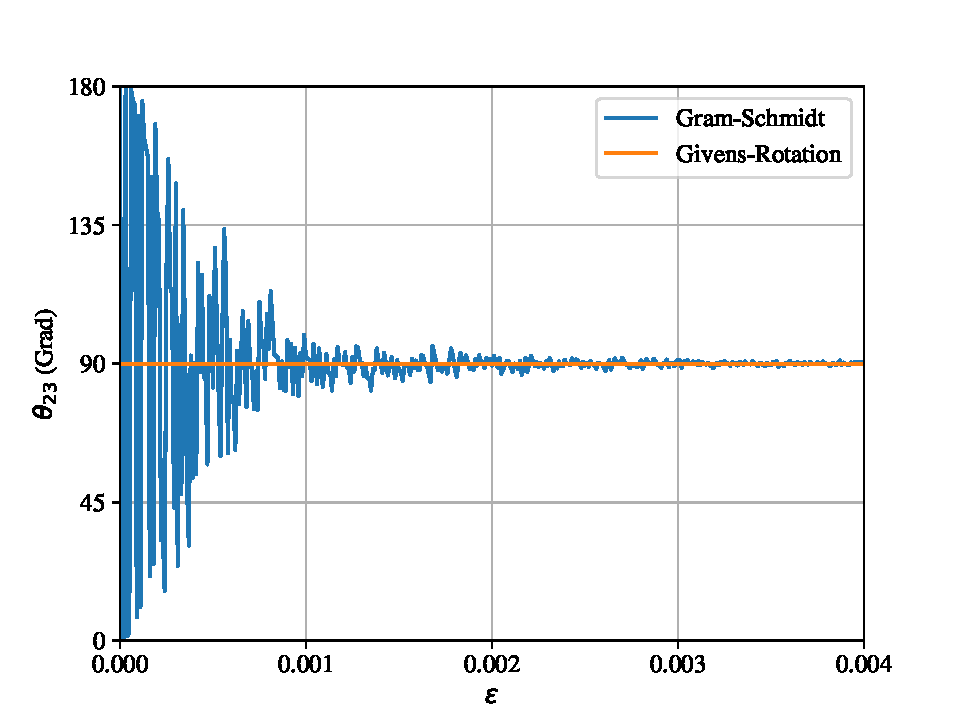
\includegraphics[width=0.9\textwidth]{papers/qr/pics/comp.pdf}
\caption{Winkel zwischen $q_2$ und $q_3$.\label{qr:comp}}
\end{figure}


Vergleich der beiden Implementationen.

Plot mit von Winkelabweichung gegenüber $\pi/2$ (\glqq Orthogonalitätsfehler \grqq{})mit verschieden $\epsilon$ als Qualitätskontrolle der Zerlegung

